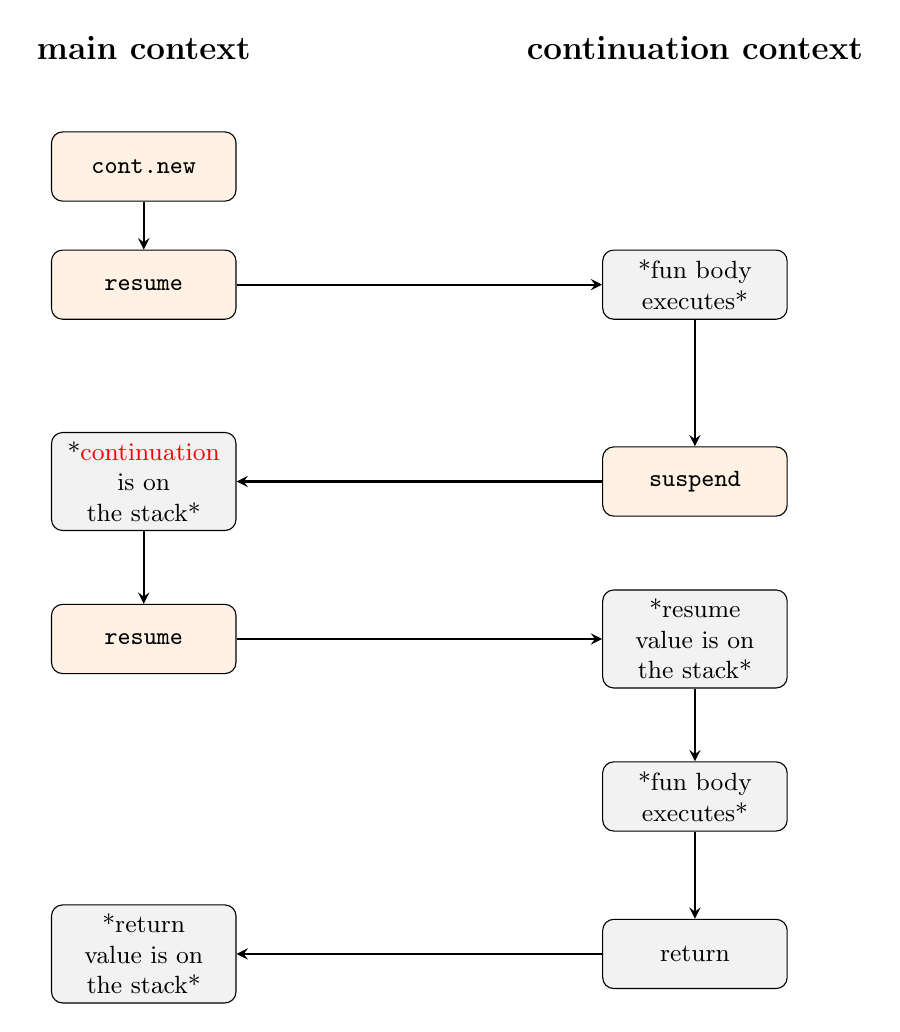
\begin{tikzpicture}[
    node distance=0.8cm and 3cm,
    every node/.style={font=\small},
    block/.style={rectangle, draw, fill=blue!10, text width=5em, text centered, rounded corners, minimum height=2.5em},
    decision/.style={diamond, draw, fill=yellow!10, text width=4em, text centered, aspect=2, inner sep=1pt},
    action/.style={rectangle, draw, fill=green!10, text width=6em, text centered, rounded corners, minimum height=2.5em},
    suspend/.style={rectangle, draw, fill=orange!20, text width=6em, text centered, rounded corners, minimum height=2.5em},
    title/.style={font=\large\bfseries},
    note/.style={rectangle, draw, fill=gray!10, text width=6em, text centered, rounded corners, minimum height=2.5em},
    primitive/.style={rectangle, draw, fill=orange!10, text width=6em, text centered, rounded corners, minimum height=2.5em},
    container/.style={rectangle, draw, fill=orange!10, text width=8em, minimum height=6em, rounded corners},
    arrow/.style={->, >=stealth, thick},
    transfer/.style={->, >=stealth, thick, dashed},
    solidarrow/.style={->, >=stealth, thick},
    label/.style={font=\scriptsize}
]
% -------------------------
% Column Titles
% -------------------------
    \node[title] (title1) at (0, 0) {main context};
    \node[title] (title2) at (7, 0) {continuation context};

% -------------------------
% Left Column Nodes (Main Context)
% -------------------------
    % Use primitive style for Wasm primitives
    \node[primitive] (n1) at (0, -1.5) {\texttt{cont.new}};
    \node[primitive] (n2) at (0, -3) {\texttt{resume}};

    % Use note style for description, correct typo "continuaion" -> "continuation"
    \node[note] (n3) at (0, -5.5) {*\textcolor{red}{continuation} is on\\the stack*};

    \node[primitive] (n4) at (0, -7.5) {\texttt{resume}};

    % Correct typo "reutrn" -> "return"
    \node[note] (n5) at (0, -11.5) {*return value is on\\the stack*};

% -------------------------
% Right Column Nodes (Suspend Function Context)
% -------------------------
    % Align this with the first resume (n2)
    \node[note] (n6) at (7, -3) {*fun body executes*};

    % Use primitive style for Wasm suspend instruction
    \node[primitive] (n7) at (7, -5.5) {\texttt{suspend}};

    % Note below n7
    \node[note] (n8) at (7, -7.5) {*resume value is on\\the stack*};

    % Note below n8
    \node[note] (n9) at (7, -9.5) {*fun body executes*};

    % Note below n9
    \node[note] (n10) at (7, -11.5) {return};

% -------------------------
% Arrows & Routing (Corrected flow from image_1.png)
% -------------------------
    \draw[arrow] (n1) -- (n2);
    \draw[arrow] (n2) -- (n6);
    \draw[arrow] (n6) -- (n7);
    \draw[arrow] (n7) -- (n3); % This transfer is from suspend context to main
    \draw[arrow] (n3) -- (n4);
    \draw[arrow] (n4) -- (n8); % This transfer is from main to suspend context
    \draw[arrow] (n8) -- (n9);
    \draw[arrow] (n9) -- (n10);
    \draw[arrow] (n10) -- (n5); % This transfer is from suspend context back to main
\end{tikzpicture}
